\chapter{Introdução}


Ao longo das últimas décadas, à medida que novos campos de petróleo e gás foram descobertos em águas profundas e distantes da costa, surgiu a necessidade de utilização de sistemas de coleta e exportação submarinos utilizando dutos rígidos cada vez mais extensos.
Com uma maior extensão, aumentou-se a ocorrência de seções de duto não suportadas, chamadas de vãos-livres, devido às irregularidades do leito marinho, sejam elas preexistentes durante a instalação ou devido a subsequentes movimentos horizontais de \textit{scouring}\footnote{retirada de solo que suporta o duto devido às intensas correntes de fundo.} de dutos durante a operação.

A presença de trechos do duto em vão-livre exige uma avaliação para determinar a necessidade de ações corretivas para evitar danos aos mesmos.
Ainda na fase de projeto, uma avaliação do perfil do fundo do mar ao longo da rota proposta pode ser realizada para identificar se é esperado que haja trechos do duto em vão-livre.
Na existência de tais trechos, será necessária uma análise que forneça previsões dos números e tamanhos dos vãos esperados, que são indicadores da necessidade de possíveis alterações na rota ou ações corretivas.

Devido aos elevados custos (ambientais, financeiros, e à imagem da empresa), associados aos acidentes, o transporte seguro de hidrocarbonetos e outros fluidos nos oleodutos é uma das principais prioridades da indústria de petróleo e gás.
A vibração livre é uma grande preocupação na análise de fadiga de componentes de dutos submarinos, incluindo dutos em vãos-livres~\cite{Gamino2013}.

Sendo assim, o comportamento estático e dinâmico do duto deve ser investigado para garantir a segurança, combatendo o dano estrutural por fadiga, mantendo-o em um estado aceitavelmente seguro.
Se as condições necessárias à segurança não puderem ser garantidas, as ações corretivas na forma de mudança de rota, correção de vãos, supressão do VIV e similares são usadas para garantir que os critérios de projeto relativos aos níveis de tensão e possíveis danos por fadiga devido ao VIV não sejam excedidos.
A análise requer o uso de métodos numéricos robustos para seu tratamento, e o Método dos Elementos Finitos (MEF) é amplamente usado nessa tarefa.
A configuração de dutos no fundo do mar depende das características topográficas do leito marinho, características do solo, tensão residual de lançamento, rigidez do duto e seu peso submerso.

Para que as condições de contorno e características do problema simulado reproduzam comportamento in loco, é necessário modelar desde a etapa de instalação até a operação do duto, assim como considerar efeito de carregamentos dos diferentes valores de pressões internas e externas nas respectivas etapas.
Modelar a instalação de dutos em um software de elementos finitos para uso geral pode ser um trabalho demorado e tedioso, principalmente devido a grandes quantidades de dados da batimetria.
Na maioria das vezes, são necessárias técnicas avançadas de \textit{script} para definir o perfil do leito marinho e simular o processo de assentamento~\cite{VandenAbeele2013}.

Nesse cenário, são essenciais ferramentas que possam auxiliar não só no processamento (como os softwares de simulação), mas também o pré e pós-processamento de dados e, até mesmo, na automação de procedimentos.
Uma ferramenta com essas características traz ganhos significativos para a produtividade e reduz a possibilidade de ocorrência de erros humanos.
Além disso, uma ferramenta que integre softwares de uso específico (para análise e visualização, por exemplo), pode reduzir atritos do fluxo de trabalho, em comparação ao uso isolado destes softwares.


\section{Soluções comerciais existentes}


No cenário mundial existe a tendência da indústria de óleo e gás de investimento em transformação digital em todas as áreas da cadeia, com desenvolvimento de práticas e ferramentas. Esse movimento levou ao surgimento de ferramentas específicas ao auxílio do profissional responsável pela análise, visualização, predição dos resultados de VIV em dutos em vão-livre~\cite{Mittal2017}. No entanto, pela especificidade dessas ferramentas, seu número ainda é reduzido, destacando apenas duas de nível comercial.


\subsection{SAGE Profile}


Desenvolvido pela empresa Fugro, que atua no monitoramento de dutos submarinos, o SAGE Profile~\cite{sageprofile} é o software deles para análise de dutos submarinos. Por ser específica para este uso, esta aplicação representa avanços em relação à modelagem com um software de elementos finitos genéricos. No entanto, ela se limita a análise de elementos finitos, deixando a análise de fadiga a cargo do usuário. Além disso, a interação do usuário está limitada a interface gráfica (GUI\footnote{\textit{Graphical User Interface}: interface de usuário gráfica}, como na \autoref{fig:sageprofile}), o que dificulta a automação de tarefas corriqueiras.

\begin{figure}[!ht]
    \centering
    \caption{Interface gráfica do SAGE Profile.}\label{fig:sageprofile}
    \begin{subfigure}[t]{0.49\textwidth}
        \centering
        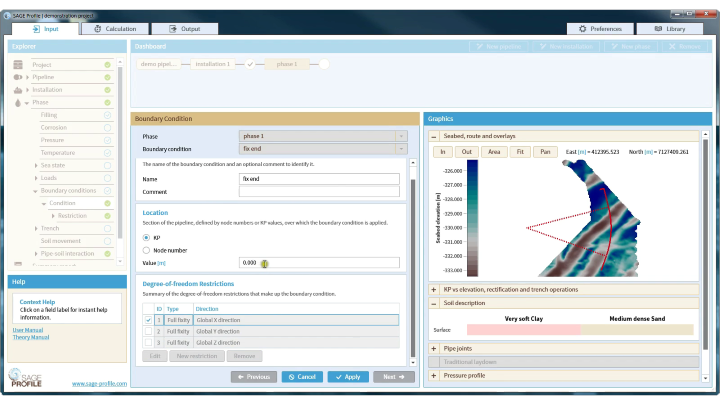
\includegraphics[width=\textwidth]{imagens/sage_profile_1}
    \end{subfigure}
    \hfill
    \begin{subfigure}[t]{0.49\textwidth}
        \centering
        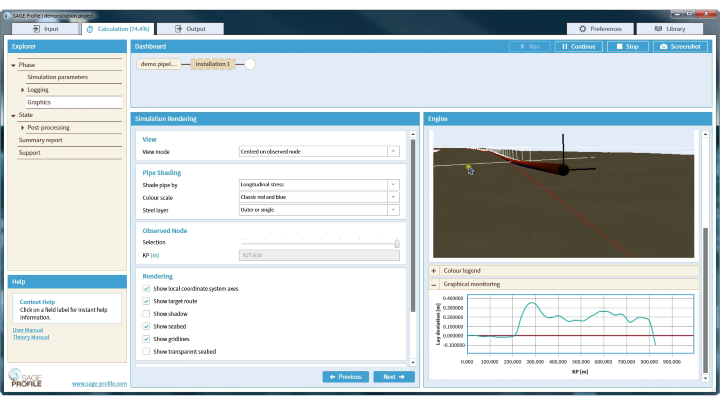
\includegraphics[width=\textwidth]{imagens/sage_profile_2}
    \end{subfigure}
    \fonte{www.sage-profile.com.}
\end{figure}


\subsection{Sesam for pipelines}

A DNG-GL é uma referência mundial, entre outras áreas, em análise de dutos em vão-livre. Esta empresa é responsável pelo desenvolvimento da suíte \textit{Sesam for pipelines}~\cite{dnvsesam} focados na análise de dutos submarinos.
Essa suíte consiste em 6 aplicações em VBA\footnote{Sigla para \textit{Visual Basic for Applications}, uma linguagem pela qual se pode customizar e extender aplicações com Microsoft.}, dentre as quais a mais destacada é a \fatfree, responsável pelo cálculo da vida a fadiga em si. Sendo desenvolvidas pela DNG-GL, as aplicações seguem as recomendações práticas propostas pela mesma --- que traz bastante confiabilidade nos resultados. Entretanto, apesar de conter uma aplicação para análise de comportamento mecânico, estas aplicações são simples, e estão muito aquém de uma solução completa para simulação assentamento do tudo no solo, como o SAGE Profile.

\begin{figure}[!ht]
    \centering
    \caption{Interface gráfica (planilha) da \fatfree.}\label{fig:fatfree}
    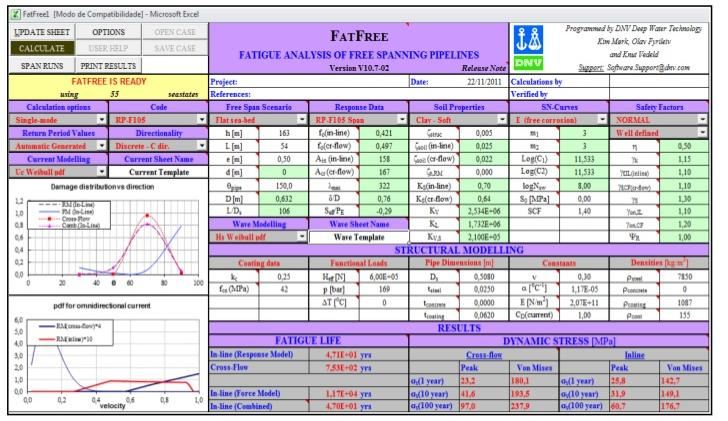
\includegraphics[width=0.8\textwidth]{imagens/fatfree}
    \fonte{Autor (2020)}
\end{figure}


\section{Motivação}


Atualmente, existem diversos sistemas submarinos em operação nas Bacias de Campos e Espírito Santo que estão no final ou já ultrapassaram a metade de sua vida útil de projeto, o que torna ainda mais relevante uma análise de integridade avaliando possibilidade de extensão de vida operacional com critérios de cálculo validados.

Como se pode ver, dentre as melhores ferramentas atuais para análise fadiga de duto em vão-livre ainda há espaço para melhorias, especialmente no que se refere a integração. Diante dessas limitações, é comum usar um software para a análise de elementos finitos genérico (como ABAQUS e ANSYS\footnote{https://www.ansys.com}) e realizam o cálculo de fadiga em folhas de cálculo pessoais ou comerciais, como a \fatfree.

Visando desenvolver uma nova ferramenta para. Portanto, um framework com o qual se possam construir aplicações para automatizar tarefas no fluxo de trabalho desde a análise de elementos finitos até análise de fadiga traria uma importante Contribuição para o panorama atual.


\section{Fluxo de avaliação de vida à fadiga sem o \frame}\label{sec:workflow}


Baseado nos estudos e oficinas realizados para o desenvolvimento deste trabalho. Pôde-se estabelecer que a análise de vida à fadiga em dutos em vão-livre compreende o fluxograma apresentado na \autoref{fig:fluxograma}. % chktex 19

\begin{figure}[!ht]
    \centering
    \caption{Fluxo de avaliação de vida à fadiga em dutos em vão-livre.}\label{fig:fluxograma}
    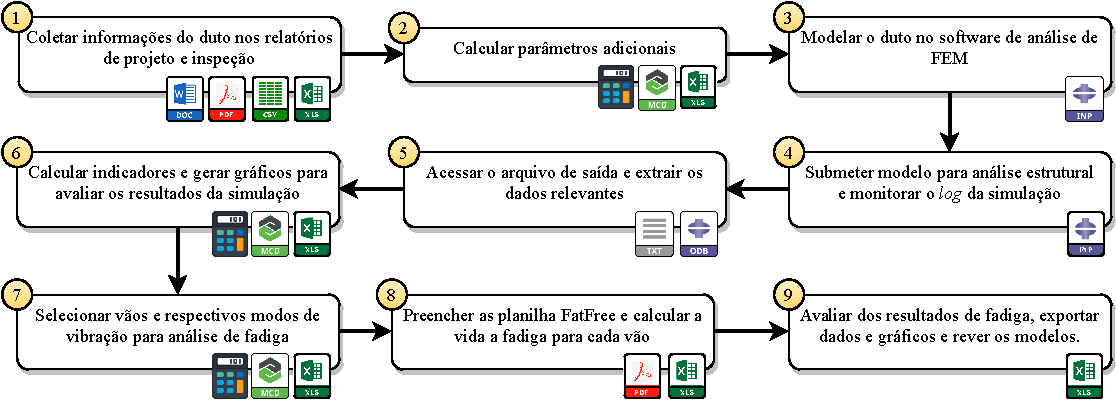
\includegraphics[width=\textwidth]{imagens/fluxograma.pdf}
    \fonte{Autor (2020)}
\end{figure}

A seguir, uma breve descrição de cada item:

\begin{enumerate}[label= (\arabic*)]
    \item Nesta etapa, o profissional reúne as informações básicas para construção dos modelos e outros dados usados em cálculos posteriores. Citadamente, temos aqui: as cotas do perfil do duto e batimetria obtidas na inspeção, geometria e propriedades dos materiais das camadas que compõem sessão do duto, parâmetros do solo, coeficientes de segurança e outras constantes físicas, posição e tipos de suportes ao longo do duto. Essa tarefa envole analisar uma série de documentos (\texttt{.doc}, \texttt{.pdf}, etc) em busca desses valores, dispostos de forma não estruturada. Quando estruturados, em forma de arquivos CSV ou planilhas, por exemplo, é necessário ainda manipular esses dados de modo a extrair somente a informação necessária e/ou convertê-las no formato apropriado. Um exemplo disso são os dados de batimetria, que precisam convertidos nas coordenadas dos nós de uma malha de elementos finitos no formato de um arquivo \texttt{.inp}.---no caso do ABAQUS. De posse desses dados, pode-se então, iniciar a fase de pré-processamento.
    \item Uma vez que nem todos os dados a serem utilizados estão de acordo com as especificações dos softwares a serem empregados nas análises numéricas, ainda é necessários manipular alguns desses valores, seja calculando constantes ou convertendo unidades. Para isso, geralmente utiliza-se softwares de planilhas e/ou folhas de cálculos (Microsoft Excel, MathCad, Maple, etc.). Esta etapa inicia o pré-processamento dos dados.
    \item Com todos os dados em mãos, é necessário transformá-los em um modelo no software de elementos finitos, via interação com mouse e teclado (GUI), ou criando arquivos de entrada. Embora a reutilização de arquivos de entrada previamente criados facilite essa tarefa, nem todos os trechos desses arquivos são suficientes ou podem ser reaproveitados. Estas limitações são frequentes em trechos do arquivo que precisam ser repetidos a depender da quantidade de certas entidades no modelo---suportes, por exemplo. Ao fim desta etapa, encerra-se o pré-processamento dos dados.
    \item Por mais simples que seja submeter o modelo para análise na maioria dos softwares de análise de elementos (alguns cliques via GUI, ou um comando via CLI\footnote{\textit{Command Line Interface}: interface de linha de comando}), as análises costumam levar horas e envolver execuções sucessivas a fim de realizar intervenções no modelo que não podem ser modeladas previamente. Dessa forma, torna-se necessário o monitoramento do progresso da simulação. Esta etapa compreende a primeira parte do processamento propriamente dito.
    \item Uma vez concluída a simulação Análise de Elementos Finitos (FEA, em inglês), é necessário analisar os resultados antes do pós-processamento. Por vezes, é preciso extrair os resultados que estão armazenados em arquivos proprietários (como \texttt{.odb}, no caso do ABAQUS), utilizando as funcionalidades das ferramentas dos próprios pacotes de software de elementos finitos para isso. Esta tarefa, geralmente feita via GUI, costuma ser repetitiva e pode levar de alguns minutos ou horas. Esta etapa inicia parte do pós-processamento da FEA\@.
    \item De posse dos resultados em formatos acessíveis a outros software (MS Excel e MathCad, por exemplo), é necessário calcular (e muitas vezes visualizar em gráficos) alguns indicadores a fim de avaliar a validade dos resultados. Embora poderosos, estes softwares ainda carecem de gráficos mais interativos, como possibilidades de ampliar e transladar os gráficos com o mouse. Esta etapa encerra o pós-processamento da FEA\@.
    \item Na metodologia presente na \dnvf105---que será abordada adiante no \autoref{sec:multimode}---o cálculo de fadiga é baseada em modelos de resposta, portanto, é necessário calcular a resposta de cada modo para as várias condições de carregamento ambiental, o que a torna impraticável sem automação. Para solucionar este problema, foi criada a \fatfree, uma planilha de cálculo comercial que realiza estas operações. No entanto, dentre as dezenas de modos obtidos por solução modal na FEA costumam aparecer modos espúrios. Dessa forma, antes de realizar a análise na \fatfree, é necessário escolher dentre os modos de vibração obtidos na simulação numérica aqueles que mais contribuem para fadiga. Esta tarefa pode ser feita via inspeção visual, observando a forma dos modos, mas é uma prática pouco precisa e subjetiva.
    \item Uma vez selecionados os modos a serem usados para cálculo de fadiga, é necessário o preenchimento da planilha com os dados de deflexão normalizada de cada modos, o que consiste em algumas centenas de valores. Além disso, é necessário preencher muitas outras informações referentes geometria e propriedades dos materiais da sessão do duto, parâmetros do solo, coeficientes de segurança e condições de carregamento em várias páginas diferentes. Com todos os dados preenchidos e opções selecionadas nos controles da planilha, pode-se apertar o botão que calcula os resultados de fadiga.
    \item Finalmente, os dados de fadiga pode ser analisados e exportados para outras ferramentas a fim de gerar relatórios.
\end{enumerate}


\section{Objetivos}


Este trabalho tem como objetivo geral desenvolver um \textit{framework} para a análise de fadiga em dutos submarinos em vãos-livres, que permita um fluxo de trabalho que inclua um software de análise de elementos finitos e uma planilha de cálculo de vida a fadiga.
Além disso, este trabalho tem como objetivos específicos:

\begin{itemize}
    \item Contribuir para a metodologia de análise de fadiga em dutos por meio da criação de uma metodologia de seleção de modos de vibração;
    \item Modelar e implementar um \textit{framework} utilizando o paradigma da programação orientada a objetos, através da linguagem \textit{Python};
    \item Validar o \textit{framework} com aplicação de casos.
\end{itemize}


\section{Delimitação do trabalho}


Este trabalho descreve o processo de desenvolvimento de um \textit{framework} para auxílio.


\section{Organização do Trabalho}

Nesta seção são apresentados, de forma resumida, os assuntos que serão tratados com mais detalhes em cada capítulo do presente trabalho. No capítulo introdutório, apresenta-se o contexto no qual o problema está inserido, bem como algumas informações relevantes para reforçar a importância do tema em estudo. Além disso, são definidos alguns conceitos iniciais a fim de garantir uma melhor compreensão do que está sendo tratado.
% TODO: E o capítulo 2???
O \autoref{chap:fundamentacao} apresenta os conceitos básicos para compressão do problema de determinação da vida à fadiga em dutos em vão-livre. Este capítulo está dividido em duas sessões. A primeira (\autoref{sec:assentamento}) apresenta a modelagem computacional do comportamento de dutos submarinos, os passos de carga, e os tipos de elementos empregados para modelar os elementos necessários a simulação. Já a \autoref{sec:viv}, apresenta os conceitos e as formulações por trás da Vibração Induzida por Vórtice (VIV), e as recomendações dados pela referência técnica \dnvf105.

O \autoref{chap:software} é apresentado o fluxo  os aspectos da implementação computacional da ferramenta, bem como os princípios norteadores de algumas escolhas, como a escolha da linguagem e paradigma de programação, a estrutura proposta para os módulos e classe.

No \autoref{chap:aplicacoes} tem-se a apresentação do uso da aplicação da ferramenta em uma análise de vida à fadiga para um caso particular. Neste capítulo é possível observar como se faz o uso das principais funções implementadas e a forma de apresentação dos resultados.

No \autoref{chap:conclusao} são tratadas as considerações finais do trabalho, bem como são apresentadas algumas sugestões para trabalhos futuros.
